\documentclass[oneside, a4paper, onecolumn, 11pt]{article}

\usepackage{amsmath, amssymb}
\usepackage{booktabs, bm}           %%  bold math
\usepackage{cancel}
\usepackage{dcolumn}  %%  Align table columns on decimal point
\usepackage{epsfig, epsf, eurosym, enumitem}
\usepackage{fancyhdr}
\usepackage[T1]{fontenc}
\usepackage[para]{footmisc}
\usepackage{graphicx }
%\usepackage{lscape}
\usepackage{hyperref,ifthen}
\usepackage{mathptmx, multicol}
\usepackage[authoryear, round]{natbib}
\usepackage{nopageno}
\usepackage{subfigure}
\usepackage{verbatim}
\usepackage{threeparttable}
\usepackage[usenames,dvipsnames]{xcolor}
\usepackage{tcolorbox}
\usepackage{tabularx}
\usepackage{array}
\usepackage{colortbl}
\usepackage{framed}
\usepackage{todonotes}



%%%%%%%%%%%%%%%%%%%%%%%%%%%%%%%%%%%%%%%%%%%
%       define Journal abbreviations      %
%%%%%%%%%%%%%%%%%%%%%%%%%%%%%%%%%%%%%%%%%%%
\def\nat{Nat} \def\apjl{ApJ~Lett.} \def\apj{ApJ}
\def\apjs{ApJS} \def\aj{AJ} \def\mnras{MNRAS}
\def\prd{Phys.~Rev.~D} \def\prl{Phys.~Rev.~Lett.}
\def\plb{Phys.~Lett.~B} \def\jhep{JHEP}
\def\npbps{NUC.~Phys.~B~Proc.~Suppl.} \def\prep{Phys.~Rep.}
\def\pasp{PASP} \def\aap{Astron.~\&~Astrophys.} \def\araa{ARA\&A}
\def\jcap{\ref@jnl{J. Cosmology Astropart. Phys.}} 
\def\nar{New~A.R.} \def\aapr{A\&ARv}

\newcommand{\preep}[1]{{\tt #1} }

%%%%%%%%%%%%%%%%%%%%%%%%%%%%%%%%%%%%%%%%%%%%%%%%%%%%%
%              define symbols                       %
%%%%%%%%%%%%%%%%%%%%%%%%%%%%%%%%%%%%%%%%%%%%%%%%%%%%%
\def \Mpc {~{\rm Mpc} }
\def \Om {\Omega_0}
\def \Omb {\Omega_{\rm b}}
\def \Omcdm {\Omega_{\rm CDM}}
\def \Omlam {\Omega_{\Lambda}}
\def \Omm {\Omega_{\rm m}}
\def \ho {H_0}
\def \qo {q_0}
\def \lo {\lambda_0}
\def \kms {{\rm ~km~s}^{-1}}
\def \kmsmpc {{\rm ~km~s}^{-1}~{\rm Mpc}^{-1}}
\def \hmpc{~\;h^{-1}~{\rm Mpc}} 
\def \hkpc{\;h^{-1}{\rm kpc}} 
\def \hmpcb{h^{-1}{\rm Mpc}}
\def \dif {{\rm d}}
\def \mlim {m_{\rm l}}
\def \bj {b_{\rm J}}
\def \mb {M_{\rm b_{\rm J}}}
\def \mg {M_{\rm g}}
\def \mi {M_{\rm i}}
\def \qso {_{\rm QSO}}
\def \lrg {_{\rm LRG}}
\def \gal {_{\rm gal}}
\def \xibar {\bar{\xi}}
\def \xis{\xi(s)}
\def \xisp{\xi(\sigma, \pi)}
\def \Xisig{\Xi(\sigma)}
\def \xir{\xi(r)}
\def \max {_{\rm max}}
\def \gsim { \lower .75ex \hbox{$\sim$} \llap{\raise .27ex \hbox{$>$}} }
\def \lsim { \lower .75ex \hbox{$\sim$} \llap{\raise .27ex \hbox{$<$}} }
\def \deg {^{\circ}}
%\def \sqdeg {\rm deg^{-2}}
\def \deltac {\delta_{\rm c}}
\def \mmin {M_{\rm min}}
\def \mbh  {M_{\rm BH}}
\def \mdh  {M_{\rm DH}}
\def \msun {M_{\odot}}
\def \z {_{\rm z}}
\def \edd {_{\rm Edd}}
\def \lin {_{\rm lin}}
\def \nonlin {_{\rm non-lin}}
\def \wrms {\langle w_{\rm z}^2\rangle^{1/2}}
\def \dc {\delta_{\rm c}}
\def \wp {w_{p}(\sigma)}
\def \PwrSp {\mathcal{P}(k)}
\def \DelSq {$\Delta^{2}(k)$}
\def \WMAP {{\it WMAP \,}}
\def \cobe {{\it COBE }}
\def \COBE {{\it COBE \;}}
\def \HST  {{\it HST \,\,}}
\def \Spitzer  {{\it Spitzer \,}}
\def \ATLAS {VST-AA$\Omega$ {\it ATLAS} }
\def \BEST   {{\tt best} }
\def \TARGET {{\tt target} }
\def \TQSO   {{\tt TARGET\_QSO}}
\def \HIZ    {{\tt TARGET\_HIZ}}
\def \FIRST  {{\tt TARGET\_FIRST}}
\def \zc {z_{\rm c}}
\def \zcz {z_{\rm c,0}}


\newcommand{\sqdeg}{deg$^{-2}$}
\newcommand{\lya}{Ly$\alpha$\ }
%\newcommand{\lya}{Ly\,$\alpha$\ }
\newcommand{\lyaf}{Ly\,$\alpha$\ forest}
%\newcommand{\eg}{e.g.~}
%\newcommand{\etal}{et~al.~}
\newcommand{\cii}{C\,{\sc ii}\ }
\newcommand{\ciii}{C\,{\sc iii}]\ }
\newcommand{\civ}{C\,{\sc iv}\ }
\newcommand{\SiIV}{Si\,{\sc iv}\ }
\newcommand{\mgii}{Mg\,{\sc ii}\ }
\newcommand{\feii}{Fe\,{\sc ii}\ }
\newcommand{\feiii}{Fe\,{\sc iii}\ }
\newcommand{\caii}{Ca\,{\sc ii}\ }
\newcommand{\halpha}{H\,$\alpha$\ }
\newcommand{\hbeta}{H\,$\beta$\ }
\newcommand{\oi}{[O\,{\sc i}]\ }
\newcommand{\oii}{[O\,{\sc ii}]\ }
\newcommand{\oiii}{[O\,{\sc iii}]\ }
\newcommand{\heii}{[He\,{\sc ii}]\ }
\newcommand{\nii}{N\,{\sc ii}\ }
\newcommand{\nv}{N\,{\sc v}\ }

%% From:: /cos_pc19a_npr/LaTeX/proposals/JWST/JWST_ERS/Proposal/lines.tex
%%  
\newcommand{\imw}{$i$--$W3$}
\newcommand{\imwf}{$i$--$W4$}
\newcommand{\rmwf}{$r$--$W4$}
\newcommand{\imwt}{$i$--$W2$}
\newcommand{\wtmwf}{$W3$--$W4$}
%\newcommand{\kms}{km s$^{-1}$}
\newcommand{\cmN}{cm$^{-2}$}
\newcommand{\cmn}{cm$^{-3}$}
%\newcommand{\msun}{M$_{\odot}$}
\newcommand{\lsun}{L$_{\odot}$}
\newcommand{\lam}{$\lambda$}
\newcommand{\mum}{$\mu$m}
\newcommand{\ebv}{$E(B$$-$$V)$}
%\newcommand{\heii}{\mbox{He\,{\sc ii}}}
\newcommand{\cv}{\mbox{C\,{\sc v}}}
%\newcommand{\civ}{\mbox{C\,{\sc iv}}}
%\newcommand{\ciii}{\mbox{C\,{\sc iii}}}
%\newcommand{\cii}{\mbox{C\,{\sc ii}}}
%\newcommand{\nv}{\mbox{N\,{\sc v}}}
\newcommand{\niv}{\mbox{N\,{\sc iv}}}
\newcommand{\niii}{\mbox{N\,{\sc iii}}}
%\newcommand{\oi}{\mbox{O\,{\sc i}}}
%\newcommand{\oii}{\mbox{O\,{\sc ii}}}
%\newcommand{\oiii}{\mbox{[O\,{\sc iii}]}}
\newcommand{\oiv}{\mbox{O\,{\sc iv}}}
\newcommand{\ov}{\mbox{O\,{\sc v}}}
\newcommand{\ovi}{\mbox{O\,{\sc vi}}}
\newcommand{\ovii}{\mbox{O\,{\sc vii}}}

%\newcommand{\feii}{\mbox{Fe\,{\sc ii}}}
%\newcommand{\feiii}{\mbox{Fe\,{\sc iii}}}
%\newcommand{\mgii}{\mbox{Mg\,{\sc ii}}}
\newcommand{\neii}{[Ne\,{\sc ii}]\ }
\newcommand{\neiii}{[Ne\,{\sc ii}]\ }
\newcommand{\nev}{Ne\,{\sc v}\ }
\newcommand{\nevi}{[Ne\,{\sc vi}]\ }
\newcommand{\neviii}{\mbox{Ne\,{\sc viii}}}
\newcommand{\aliii}{\mbox{Al\,{\sc iii}}}
\newcommand{\siii}{\mbox{Si\,{\sc ii}}}
\newcommand{\siiii}{\mbox{Si\,{\sc iii}}}
\newcommand{\siiv}{\mbox{Si\,{\sc iv}}}
%\newcommand{\lya}{\mbox{Ly$\alpha$}}
%\newcommand{\lyb}{\mbox{Ly$\beta$}}
\newcommand{\hi}{\mbox{H\,{\sc i}}}
\newcommand{\snine}{\mbox{[S\,{\sc ix}]}}
\newcommand{\sivi}{\mbox{[Si\,{\sc vi}]}}
\newcommand{\sivii}{\mbox[{Si\,{\sc vii}]}}
\newcommand{\siix}{\mbox{[Si\,{\sc ix}]}}
\newcommand{\six}{\mbox{[Si\,{\sc x}]}}
\newcommand{\sixi}{\mbox{[Si\,{\sc xi}]}}
\newcommand{\caviii}{\mbox{[Ca\,{\sc viii}]}}
\newcommand{\arii}{\mbox{[Ar\,{\sc ii}]}}

%%[Ar II] 6.97
%% [S IX] 1.252 μm 328 
% [Si X] 1.430 μm 351 
% [Si XI] 1.932 μm 401 
% [Si VI] 1.962 μm 167 
% [Ca VIII] 2.321 μm 128 
% [Si VII] 2.483 μm 205 
% [Si IX] 3.935 μm 303
% [Ar II] 6.97


%\snine\ at 1.252$\mu$m, \six\ at 1.430$\mu$m, \sixi\ at 1.932$\mu$m, \sivi\ at
%1.962$\mu$m, \caviii\ at 2.321$\mu$m, \sivi\ at 2.483$\mu$m \siix\ at
%3.935$\mu$m and \arii\ at 6.97$\mu$m. 
%%
%% such as [Ne ii]12.8 μm, [Ne v]14.3 μm, [Ne iii]15.5 μm, [S iii]18.7 μm and 33.48 μm, [O iv]25.89 μm and [Si ii]34.8 μm (e.g
%%
%% MIR emission lines like [NeII] and [NeV] are ..
%%
%% Also,  arXiv:astro-ph/0003457v1 
%% [NeV] 14.32um & 24.32um and [NeVI] 7.65um imply an A(V)>160 towards the NLR...
%% [NeIII]15.56um/[NeII]12.81um
%%
%% [Ne V] 14.3, 24.2 μm 97.
%% [Ne II] 12.8 μm
%% [OIV] 26μm
%%


\usepackage[left=2.05cm,top=2.05cm,right=2.05cm]{geometry}
\setlength{\bibsep}{0.0pt}

%% To fix list things: 
\setitemize{noitemsep,topsep=0pt,parsep=0pt,partopsep=0pt,leftmargin=*}

\pagestyle{fancy}
%\renewcommand{\headrulewidth}{0pt}      %% Remove line at top

%\pagestyle{empty}
\fancyhf{}
\lhead{{\it Ross}}
\chead{Part B1}
\rhead{Q4D}
\setcounter{page}{1}
\lfoot{{\it ERC-COG-2018}}
\rfoot{{\it Extended Synopsis}}
\cfoot{{\it Page \thepage\ of 5}}

\newenvironment{itemize*}%
  {\begin{itemize}%
    \setlength{\itemsep}{0pt}%
    \setlength{\parskip}{0pt}}%
  {\end{itemize}}


\begin{document}

\vspace{-16pt}

\smallskip
\smallskip
\noindent
{\bf{\textcolor{Cerulean}{a. Extended Synopsis}}} 
\vspace{6pt}

\noindent
\large
{\bf{\textcolor{Cerulean}{Overview and Objectives}}}
\normalsize

%\smallskip
\noindent
Current theories of galaxy formation and evolution strongly suggest
that central, supermassive black holes (SMBHs) have a profound effect
on the galaxies that they live in \citep[e.g., ][]{KormendyHo2013}.
This is not surprising since the potential energy associated with mass
accretion onto a supermassive black hole is comparable to that
generated via the nuclear fusion in the galaxy's stars \citep[see
e.g. ][]{Fabian2012}. Thus when a galaxy goes through a ``quasar
phase'' (where gas is supplied and accreted by the SMBH) there is
ample energy to potentially impact the host galaxy and the surrounding
intergalactic medium.

\smallskip
\smallskip
\noindent
However, the critical details of the physical processes involved in
how this energy escapes the inner most regions of the galaxy and then
interacts with the gas, dust, stars and dark matter, is currently
poorly understood. This fact, along with current observational data
giving more puzzles than clues is preventing the field from moving
forward. Significant further issues arise since startling new
observations from my (Nicholas P. Ross; NPR) research team
\citep{MacLeod2016, Ross2018} show that {\it quasars vary
significantly on timescales of weeks to months}, whereas the accretion
disks (that supply `fuel' for the quasar) should take thousands of
years to change their optical emission; this has recently been called
the ``Quasar Viscosity Crisis'' \citep[e.g., ][]{Lawrence2018}. Thus,
it is unclear if we have an understanding of a physical phenomena
prevalent in many astrophysical systems: the accretion disk.

\smallskip
\smallskip
\noindent
The field of observational extragalactic astrophysics is poised for a
fundamental and rapid change. Starting in late 2019, a fleet of new
telescopes, instruments and missions will be commissioned, start data
taking, and will leap-frog the quality and quantity of data we have
available today. These surveys and missions include: the fifth
incarnation of the Sloan Digital Sky Survey
(SDSS-V\footnote{\href{www.sdss.org/future/}{{\tt
www.sdss.org/future/}}}); the Large Synoptic Survey Telescope
(LSST\footnote{\href{lsst.org}{{\tt lsst.org}}}); the Dark Energy
Spectroscopic Instrument (DESI\footnote{\href{desi.lbl.gov}{{\tt
desi.lbl.gov}}}) survey; the 4-metre Multi-Object Spectroscopic
Telescope (4MOST\footnote{\href{4most.eu}{{\tt 4most.eu}}}) survey,
and the ESA {\it Euclid}
mission\footnote{\href{sci.esa.int/euclid/}{{\tt
sci.esa.int/euclid/}}}. Even more imminent is the launch of the {\it
James Webb Space Telescope} (JWST\footnote{\href{jwst.stsci.edu}{{\tt
jwst.stsci.edu}}}).

\smallskip
\smallskip
\noindent
{\it Quasars in the 4th Dimension} (Q4D) has two broad and well-posed goals. First, we aim to
elucidate in detail {\bf how the energy directly associated with a
supermassive black holes impacts the universal galaxy population.} We
will gain a deep understanding into the physical mechanisms related to
central engine black holes; their accretion disk physics, their
dynamics on both human and galactic timescales and the role they might
play in forming and regulating the galaxy population.  Second, we
anticipate {\bf the discovery of brand new extragalactic phenomena.}
By tapping into the massive raw discovery space that the new
experiments will open up, there is the highly likely outcome of
discovering something ``brand new'' \citep{Ivezic2008,
LSST_ScienceBook}, e.g. the EM counterparts to mergers of Binary SMBHs
(with their associated gravitational wave chirp and ringdown), objects
potentially similar to repeating fast radio bursts \citet{Spitler2016}
or more objects akin to the still unexplained `SCP 06F6'
\citep{Barbary2009}.  Q4D objectives are:
\begin{enumerate}
  \item Characterize the variable extragalactic universe and quasar population. 
  \item Establish the energy transport mechanisms associated with the``quasar phase'', and explain the relation between accretion rate, black hole mass build-up with observed light curve and spectral properties. 
  \item Develop and then link theoretical accretion and galaxy formation models for a fully holistic theory of active galaxies. 
  \item Discover new extragalactic variable objects. 
\end{enumerate}

\smallskip
\smallskip
\noindent
We will achieve this by leveraging several of the new, large-scale
surveys that will all have `First Light' over the lifetime of the
project.  These critical observations are made by exploiting the large
imaging and spectroscopic datasets that will be available from the
SDSS-V, DESI, 4MOST, LSST and ESA {\it Euclid}. {\bf Crucially,
although these projects individually will deliver new state-of-the-art
datasets, it is my project that will be the first to break down the
associated data silos and combine these data in order to go beyond the
state-of-the-art.}


\medskip
\medskip
\noindent
\large
{\bf{\textcolor{Cerulean}{1. Current State of the Art.}}}
\normalsize

\smallskip
\noindent
The current state-of-the-art data samples have either
$\approx$10$^{6}$ quasars with one spectral epoch, or only a few
objects with repeat photometric data, i.e. light-curve information and
the accompanying repeat spectra (see Figure~\ref{fig:J110057}).  NPR
has been involved in the production of both of these two types of
samples \citep{MacLeod2016, Paris2017}. We plan to collate datasets so
that the 10$^{6}$ sample have {\it high-fidelity light-curves and
ample repeat spectroscopy (necessary of emission/absorption line
diagnostics}, and in doing so will kick start the new field of
Variable Extragalactic Astrophysics.

\begin{figure}[h]
  \begin{center}
    \hspace{-0.5cm}
    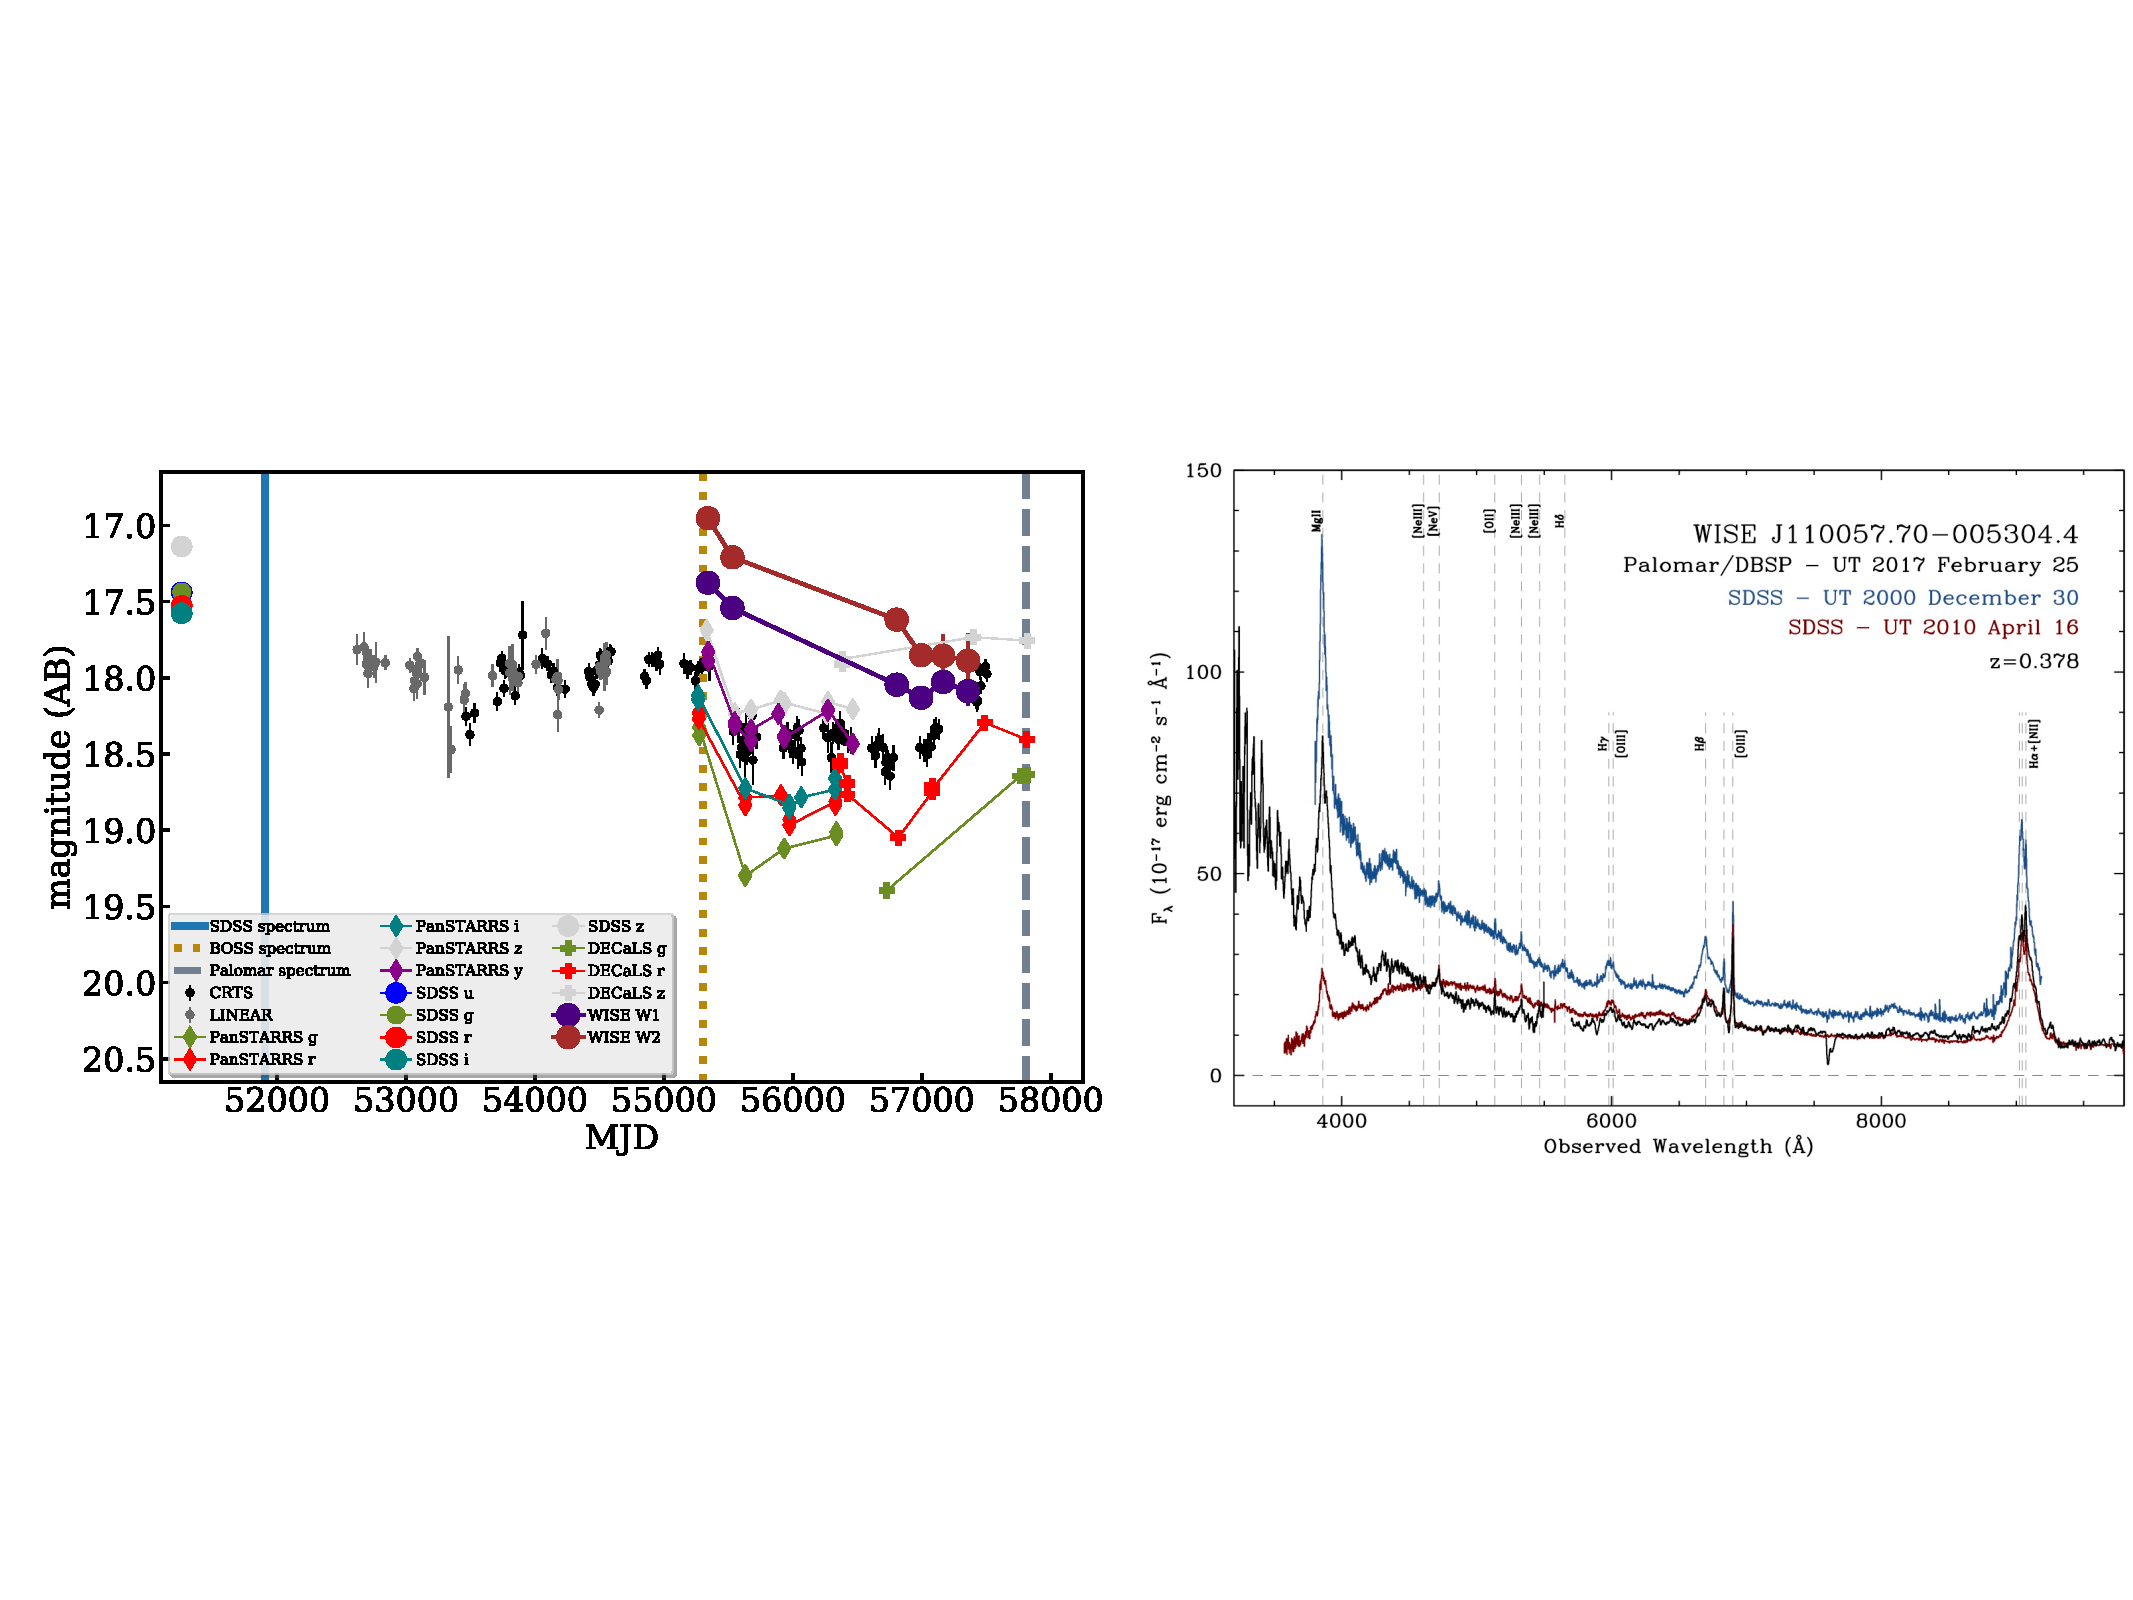
\includegraphics[height=6.25cm,width=17.2cm]
    {figures/J110057_LC_Spectra_20171024.pdf}
    \vspace{-10pt}
    \caption{\small    % \footnotesize       % \scriptsize      % \tiny
      {\it (Left:)} The optical and infrared light-curve for the redshift $z=0.378$ quasar 
      J1100-0053 (Ross et al. 2018). 
      Note the fall in the infrared, whereas there is a decrease, but 
      then recovery in the optical. 
      {\it (Right:)} 
      Three epochs of spectra for J1100-0053. 
      The spectacular downturn in the blue for the 2010 spectrum 
      indicates a dramatic change in the accretion disk.
    }
  \vspace{-22pt}
 \label{fig:J110057}
\end{center}
\end{figure}


\smallskip
\smallskip
\noindent
During its initial phases of operation the Sloan Digital Sky Survey
(SDSS) obtained spectra of 1 million galaxies in the local
Universe. This dataset has become the {\it de facto} standard for
understanding the present day galaxy population, and sets the boundary
conditions for all theoretical comparisons. The paradigm changing
success of the SDSS was due to having 1,000,000 objects {\it with very
high signal-to-noise photometry and spectra}, enabling multivariate
analysis that is required for galaxy astrophysics investigations.
{\it Q4D will generate the same sample size and revolutionary
understanding with a new temporal dimension of the quasar population,
as the SDSS had with the low-redshift $z\sim0.1$ galaxy population.}
The ground-breaking aspect of Q4D is that it takes quasar astrophysics
into the 2020s, going from single objects samples, to surveys and
samples of millions of objects, with massive spectroscopic monitoring
giving access to the time-domain and leveraging these very large scale
next generation missions, telescopes and their datasets.


\begin{figure}[h]
  \begin{center}
   \hspace{-0.5cm}
%   trim=l b r t
    \includegraphics[width=15.0cm] %, trim={0.05cm 0 0.05cm 0},clip]
    {figures/Timelines_and_Facilites.pdf}
    \vspace{-10pt}
   \caption{\small       
     Facilites, Timelines and Priorities. With SDSS-V and DESI in the Northern Hemisphere and 
     4MOST, LSST in the South, we have full celestial sphere coverage.}
  \vspace{-22pt}
 \label{fig:Keynote_facilites}
\end{center}
\end{figure}

\smallskip
\smallskip
\noindent
{\it The timing for this proposal could not be better.}  The first of
the data ``firehoses'' turns on in late 2019, with the full datastream
from our key sources fully online by mid-2022. As such, we have the
time to mature our analysis techniques, and then be in the ideal
position to take advantage of the initial data releases of all these
new projects.
%%
Prompt ERC Consolidator level-support is also imperative since final
survey design and optimization trade-off studies are being made
e.g. for DESI, SDSS-V and LSST over the next $\sim$12-18
months. Having the ability to influence and fully optimise these
decisions for our science objectives would be very powerful.  The
ground breaking nature of the Q4D will attract high quality PDRAs, 
{\it who would be guaranteed ``First Light'' data and science.}

\smallskip
\smallskip
\noindent
The importance of this branch of astrophysics is already well
established in Europe and is a priority for the next two
decades.\footnote{\href{http://sci.esa.int/cosmic-vision}{ESA Cosmic
Visions}}\footnote{\href{http://sci.esa.int/cosmic-vision/42369-l-class-timeline/}{L-Class
Mission Timeline}} This is demonstrated by noting that one of the two
primary mission goals for the ATHENA mission is answering the question
``How do black holes grow and shape the Universe?''.  ATHENA is ESA's
second L-class flagship mission, due for launch in 2028.

\smallskip
\smallskip
\noindent
{\it The scope and remit of an ERC Consolidator grant will allow us to
combine these data products in a manner that will not only establish
the new state-of-the-art in variable extragalactic astrophysics, but it 
will also establish and kickstart the new field of variable extragalactic
astrophysics itself.}




\medskip
\medskip
\noindent
\large
{\bf{\textcolor{Cerulean}{2. Methodology}}}
\normalsize

\noindent
Our proposal contains six work packages that fall into three broad and
complementary categories: observational studies of large numbers
(millions) of objects; high-risk, very high-reward observational
studies of a small number (10s) of objects; theoretical modeling
investigations. Figure~\ref{fig:workplan} summarises our overall WP
plan. Risks and mitigation strategies are present for each WP as are
Key Deliverables.  NPR, three PDRAs, ``PDRA1'', ``PDRA 2'', ``PDRA
3'', and one PhD student, ``PhD1'' are the personnel required to carry
out these work packages.


\smallskip
\smallskip
\noindent
NPR is a world-leader in the field of extragalactic observational
astrophysic. NPR's research focuses on implementing novel data
science and machine learning algorithms and techniques in order to
discover and study the physical processes in quasars. I have an
exceptionally strong track record including being the lead of a
science Working Group, with prodigious scientific output
(\href{https://tinyurl.com/ycxd8lb6}{over 400 published, peer-reviewed
papers} from that particular collaboration).
%\smallskip \smallskip \noindent
{\bf I was the Co-Founder and Chief Data Scientist of String Security
Inc. where I built a predictive threat detection and remediation
platform for cyber security teams by applying machine learning and
predictive algorithms.  Thus the P.I.'s research strengths, ability to
quickly develop bleeding-edge software and science output are all
ideally matched to this proposal.}


\smallskip
\smallskip
\noindent
The skill set of PDRA1 would include development of the underlying
tools and techniques necessary to extract meaning from large and/or
complex data sets.  PDRA1 would have a strong physical sciences
background, and a PhD in astrophysics or computer science.
%\smallskip \smallskip \noindent
The skill sets of PDRA2 would include expertise in time series
analysis, primarily with optical data but potentially also in other
wavebands.  PDRA2 would have a PhD in astrophysics or a related field.
%\smallskip \smallskip \noindent
The skill set of PDRA3 would include experience with fluid mechanics
modelling and/or large computer simulations.  PDRA3 would have a PhD in astrophysics,
mathematics or computer science.
% \smallskip \smallskip \noindent
PhD1 would have a Masters or a strong 4-year undergraduate degree in
Physics or Mathematics with evidence of research-level project work.

\begin{figure}
  \begin{center}
   \hspace{-0.5cm}
%   trim=l b r t
    \includegraphics[width=16.0cm] %, trim={0.05cm 0 0.05cm 0},clip]
    {figures/workplan.pdf}
    \vspace{-10pt}
    \caption{ \small
      An overview of the WPs, with the personnel attached to each WP
      and a guide to their start and duration. As given by the
      shadings, WP1, 2 and 3 are observational studies of large numbers of
      objects; WP4 are theoretical modeling investigations and WP5 and 6 are
      high-risk, very high-reward observational studies of small numbers of
      objects.}
  \vspace{-22pt}
 \label{fig:workplan}
\end{center}
\end{figure}


\smallskip
\smallskip
\noindent
\textbf{\textsc{WP1: Build QuasarSieve:}} 
In order to utilize the LSST datastream for our science goals we will
build a ``Stage 2 filter'', which we name {\it QuasarSieve}.  This
will identify the quasars, add context, perform outburst forecasting
etc.  The heavy-industry computing infrastructure is being supplied by
the UK LSST Data Access Center (DAC, based at the University of
Edinburgh) and our task will be to build software in a timely and
robust manner.  This is a novel enterprise and a rate-limiting step in
our overall programme, with the associated high-risk.  We mitigate
this risk with the data science and machine learning experience from
PDRA1 and the P.I. (NPR).  We thus classify {\bf WP1 as medium-risk,
high-reward.}  {\bf Key Deliverables:} An open-source, well-documented
software package that can interact with and return data from the LSST
Data Access Center.


\smallskip
\smallskip
\noindent
\textbf{\textsc{WP2: Quasar Catalogue Generation and Demographic studies:}}  
Building the quasar corpus and cataloguing the observational data will
be a vital step for our science goals.  Following on from the quasar
catalogue generation, a key science output will be the study of the
quasar demographics.  All these are vital observational tests for
galaxy formation models and theory (see WP4 below). The goal of this
WP is to construct a quasar catalogue and make key observational
tests.  Given the P.I.s experience at these specific tasks, plus the
effort level of PDRA1, PDRA2 and PhD this WP is deemed medium-risk.
{\bf WP2 is medium-risk, high-reward.}  {\bf Key Deliverables:} A
science-enabling compendium that will be the state-of-the-art quasar
dataset for the 2020s.  A suite of new, beyond-the-state-of-the-art
quasar demographic measurements which are the boundary conditions for
theoretical models.


\smallskip
\smallskip
\noindent
\textbf{\textsc{WP3: Light-Curve and Spectral Analyses:}} 
Another major scientific output will be the full and detailed light-curve
and spectral analyses of the conglomerate datasets.  This WP will have
a data science/machine learning aspect.  The goal of this WP is to
elucidate the physical processes that drive quasar variability and as
such is significant high-reward science.  This level of investigation
is highly novel, though we envisage no major barriers outside of our
control to achieving our science goals and PDRA1, PDRA2, as well as
the P.I. (NPR) and PhD1 effort will be directed towards this.  As
such, {\bf WP3 as medium-risk, high-reward.}  {\bf Key Deliverables:}
Measurements, for the first time of how the light-curves and spectra
of quasars depend on key physical quasar properties e.g. $M_{\rm
SMBH}$, luminosity, $\lambda = \log (L / L_{\rm Edd})$, spin etc.
These measurements will allow us to make direct comparisons to
accretion disk models.


\smallskip
\smallskip
\noindent
\textbf{\textsc{WP4: Accretion Disk and Quasar Feedback Simulations:}} 
New accretion models are needed to fully explain the ``changing look'' quasars 
and the ``Quasar Viscosity Crisis''. New radiation MHD codes begin to
explain the observations here, but further development is needed to
gain the desired deep understanding. Cosmological-scale 
simulations with stellar and quasar feedback are now also online. The
exceedingly ambitious goal of WP5 is to develop new holistic accretion
disk-to-cosmological scale simulations that explain our observational
results and links them to ``quasar feedback''.  WP4 is thus high-risk
due to its novel nature and algorithmic complexity.  We also envisage
ramp-up time to get our theoretical simulations to the level that will
be required by our beyond-the-state-of-the-art dataset.  However, we
mitigate this risk first by noting this will be the lead WP and top
priority for PDRA3.  We further mitigate this risk by invoking
collaboration with accretion disk theorist Prof. Ken Rice (WKMR; Chair
of Computational Astrophysics at the IfA, University of Edinburgh) and 
cosmological simulation expert 
Prof. Romeel Dave (RSD; Chair of Physics at the IfA, University of
Edinburgh).
%%
Thus PDRA3, NPR, with guidance from
WKMR and RSD would collaborate on this WP.  We thus classify {\bf WP4
as medium-to-high risk, very high-reward.}  {\bf Key Deliverables:}
New accretion disk models and theory that explain the light curve data
of our beyond-the-state-of-the-art dataset.  New galaxy evolution
models, describing the hydrodynamics involved on galactic scales, but
related to the quasar central engine.


\smallskip
\smallskip
\noindent
\textbf{\textsc{WP5: Observations of Quasars by the James Webb Space Telescope:}} 
What are the star-formation properties of luminous quasars at the peak
of quasar activity?  We aim to answer this by looking for the presence
of polycyclic aromatic hydrocarbon (PAH) spectral features in infrared
bright quasars with the {\it James Webb Space Telescope} (JWST).  {\bf
WP5 is high risk, high-reward.}  This is an ideal investigation for
the JWST, but we classify this as high-risk since we have to apply for
the telescope time and are not guaranteed the data.  We note this WP
does not impact in any direct way the other WPs and would lead to
very-high gain science.  {\bf Key Deliverables:} State-of-the-art data
products from the JWST, with the observational evidence and physical
interpretation of how ``quasar feedback'' regulates galaxy formation
in high-redshift quasars.


\smallskip
\smallskip
\noindent
\textbf{\textsc{WP6: New Object Discovery:}} 
The LSST will scan the sky repeatedly, enabling it, and us, to both
discover new, distant transient events and to study variable objects
throughout our universe. The most interesting science to come may well
be the discovery of new classes of objects. Suffice to say, this would
be exceptionally high-reward.  {\bf WP6 is high risk, exceptionally
high-reward.}  We class this as high risk, since it is complex to
class a WP with essentially unknown discovery potential as `low-risk'.
However, we {\it nota bene} that a lack of any novel discovery here
would be a startling null result.  {\bf Key Deliverables:} Potential
discovery of new classes of astronomical objects.



\smallskip \smallskip
\smallskip \smallskip
\noindent
\large
{\bf{\textcolor{Cerulean}{3. Resources,  Survey `buy-in' and Budget}}}
\normalsize

\smallskip
\smallskip
\noindent
\textbf{\textsc{Personnel:}} 
We request the resources and support for 100\% of the time and effort
for the P.I. We request the resources and support for 3 Postdoctoral
Research Associates (PDRAs), for a total of 10 PDRA year equivalents
(3+3+4). We request the resources and support for 1 PhD studentship.


\smallskip
\smallskip
\noindent
\textbf{\textsc{Survey Buy-in:}} 
We request support for the ``buy-in'' to two of the new surveys,
SDSS-V and DESI. The costs here are \euro184,100 for SDSS-V and
\euro200,100 for DESI.  We ask this support to come from the
``additional funds that can be made available to cover access to large
facilities.''  We request access to these funds as it
gives our project access to telescopes and data in the North and
South Hemispheres for complete coverage of the celestial sphere 
and delivers the crucial early spectroscopy that will be vital to
train, test and build our data science and machine learning codes and
algorithms.  We emphasise that the science return is `exponentially'
dependent on the breadth of data available and heralds a brand new regime of ``several-survey'' or
``multi-mission'' astronomy.  {\it Buy-in here would place the
P.I. and the University of Edinburgh as the only group and institute
in the world to be involved in SDSS-V, DESI, 4MOST, LSST and ESA {\it
Euclid} and JWST}.

\smallskip
\smallskip
\noindent
\textbf{\textsc{Computing Requirements:}} 
With the availability of the facilities at an institute (e.g. IfA
Cullen), university
(e.g. \href{https://www.ed.ac.uk/information-services/research-support/research-computing/ecdf}{Edinburgh
Compute and Data Facility}) and at a national
{\href{https://www.hartree.stfc.ac.uk/Pages/home.aspx}{(The Hartree
Centre)} level, the rate limiting factor will be how quickly and
efficiently we can deploy our codes and analysis. 


\smallskip
\smallskip
\noindent
\textbf{\textsc{Travel:}} 
We request support for travel for all 5 members of the group,
including repeat medium-term (i.e., few weeks) travel to the US and
ESO Chile to work with key collaborators at critical timings for the
First Light of the new telescopes.




\newpage
%%\thispagestyle{empty}
\fancyhf{}
%\lhead{{\it ERC-2018-CoG}}
%\lhead{{\it DEQUASARS: Part B1 }}
\lhead{{\it Ross}}
\chead{Part B1}
\rhead{Q4D}
\setcounter{page}{1}
\lfoot{{\it ERC-2018-CoG}}
\rfoot{{\it Extended Synopsis}}
%\cfoot{{\it Page \thepage\ of 5}}

\bibliographystyle{plainnat}
\bibliography{/cos_pc19a_npr/LaTeX/tester_mnras}

%\newpage
\begin{center}
\medskip
 \medskip
 {\large \bf References}
    \vspace{-10pt}
\end{center}
\begin{multicols}{2}[]
\noindent
%\footnotesize
%\scriptsize
%\tiny
\lbrack 1\rbrack Kormendy \& Ho, 2013, ARAA, 51, 511\\
\lbrack 2\rbrack Kormendy,  2016, ASSL, 418, 431\\
\lbrack 3\rbrack Alexander et al., 2012, NewAR, 56, 93\\
\lbrack 4\rbrack King \& Pounds, 2015, ARAA, 53, 115 \\
\lbrack 5\rbrack Heckman \& Best, 2014, ARAA, 52, 589\\
\lbrack 6\rbrack Naab \& Ostriker, 2017, ARAA, 55, 59 \\
\lbrack 7\rbrack Netzer, 2015, ARAA, 53,  365\\
\lbrack 8\rbrack Padovani, 2017, A\&ARv, 25, 2\\
%%
\lbrack  9\rbrack Ata et al., 2017, arXiv1705.06373v2\\
\lbrack10\rbrack Solsar et al., 2013, JCAP, 04, 026 \\
\lbrack11\rbrack Busca et al.,  2013, A\&A, 552, 96 \\
\lbrack12\rbrack Delubac et al.,  2015, A\&A, 574, 59 \\
\lbrack13\rbrack Bautista et al., 2017, A\&A, 603, 12 \\
\lbrack14\rbrack du Mas des Bourboux et al., 2017, arXiv1708.02225v3\\
\lbrack15\rbrack Font-Riber et al., 2014, JCAP, 05, 027\\
%%
\lbrack16\rbrack Ross et al. 2015, MNRAS, 453, 3932\\
\lbrack17\rbrack Wright et al., 2010, AJ, 140, 1868\\
\lbrack18\rbrack Zakamska et al., 2016, MNRAS, 459, 3144\\
\lbrack19\rbrack Hamann et al., 2017, MNRAS, 464, 3431\\
%%
\lbrack20\rbrack Timlin, Ross et al., 2016, ApJS, 225, 1\\
\lbrack21\rbrack Timlin, Ross et al., 2017, ApJ, {\it in prep.}\\
%%
\lbrack22\rbrack LaMassa et al., 2015, ApJ, 800, 144\\
\lbrack23\rbrack Runnoe et al., 2016, MNRAS, 455, 1691\\
\lbrack24\rbrack Ruan et al, 2016, ApJ, 826, 188\\
\lbrack25\rbrack MacLeod, Ross et al., 2016, MNRAS, 457, 389\\
%%
\lbrack26\rbrack Meisner et al., 2017, AJ, 153, 38 \\
\lbrack27\rbrack Meisner et al., 2017, AJ, 154, 161 \\
% Meisner  et al., 2017, arXiv1710.02526v1 \\
\lbrack28\rbrack Ross et al., 2017, Nat.As., {\it in prep.} \\
%%
\lbrack29\rbrack Hopkins et al., 2006, ApJS, 163, 1\\
%%
\lbrack30\rbrack Schlegel et al., 2011,  arXiv:1106.1706v2 \\
%
\lbrack31\rbrack Ross et al., 2009, ApJ, 697, 1634 \\
%%
\lbrack32\rbrack Lombriser \& Taylor, 2016, JCAP, 03, 031 \\
\lbrack33\rbrack Baker et al, 2017,  arXiv1710.06394v1 \\
%%
\lbrack34\rbrack Watson et al.,  2011, ApJ, 740, L49\\
\lbrack35\rbrack King et al., 2014, MNRAS, 441, 3454\\
\lbrack36\rbrack King et al., 2015, MNRAS, 453, 1701\\
\lbrack37\rbrack Shen et al., 2015, ApJS, 216, 4\\
%\lbrack37\rbrack The Pierre Auger Collaboration, 2017, Science, 357, 6357 \\
\lbrack38\rbrack Hviding et al.,  2017, arXiv1711.01269v1 



\end{multicols}



\end{document}
